\chapter{Projeto}

(dar um nome melhor pra seção de solução escolhida)


\section{Esquema Elétrico}
Na área de atuadores, foi realizada uma análise do esquema elétrico fornecido pelo professor. A partir disso, verificaram-se as conexões da porta paralela, assim como os componentes e conexões utilizados. Abaixo estão as imagens do esquema original (Fig. \ref{fig:prof_schematic}) e do desenvolvido no KiCad (Fig. \ref{fig:kicad_schematic}).

\begin{figure}[H]
    \centering
    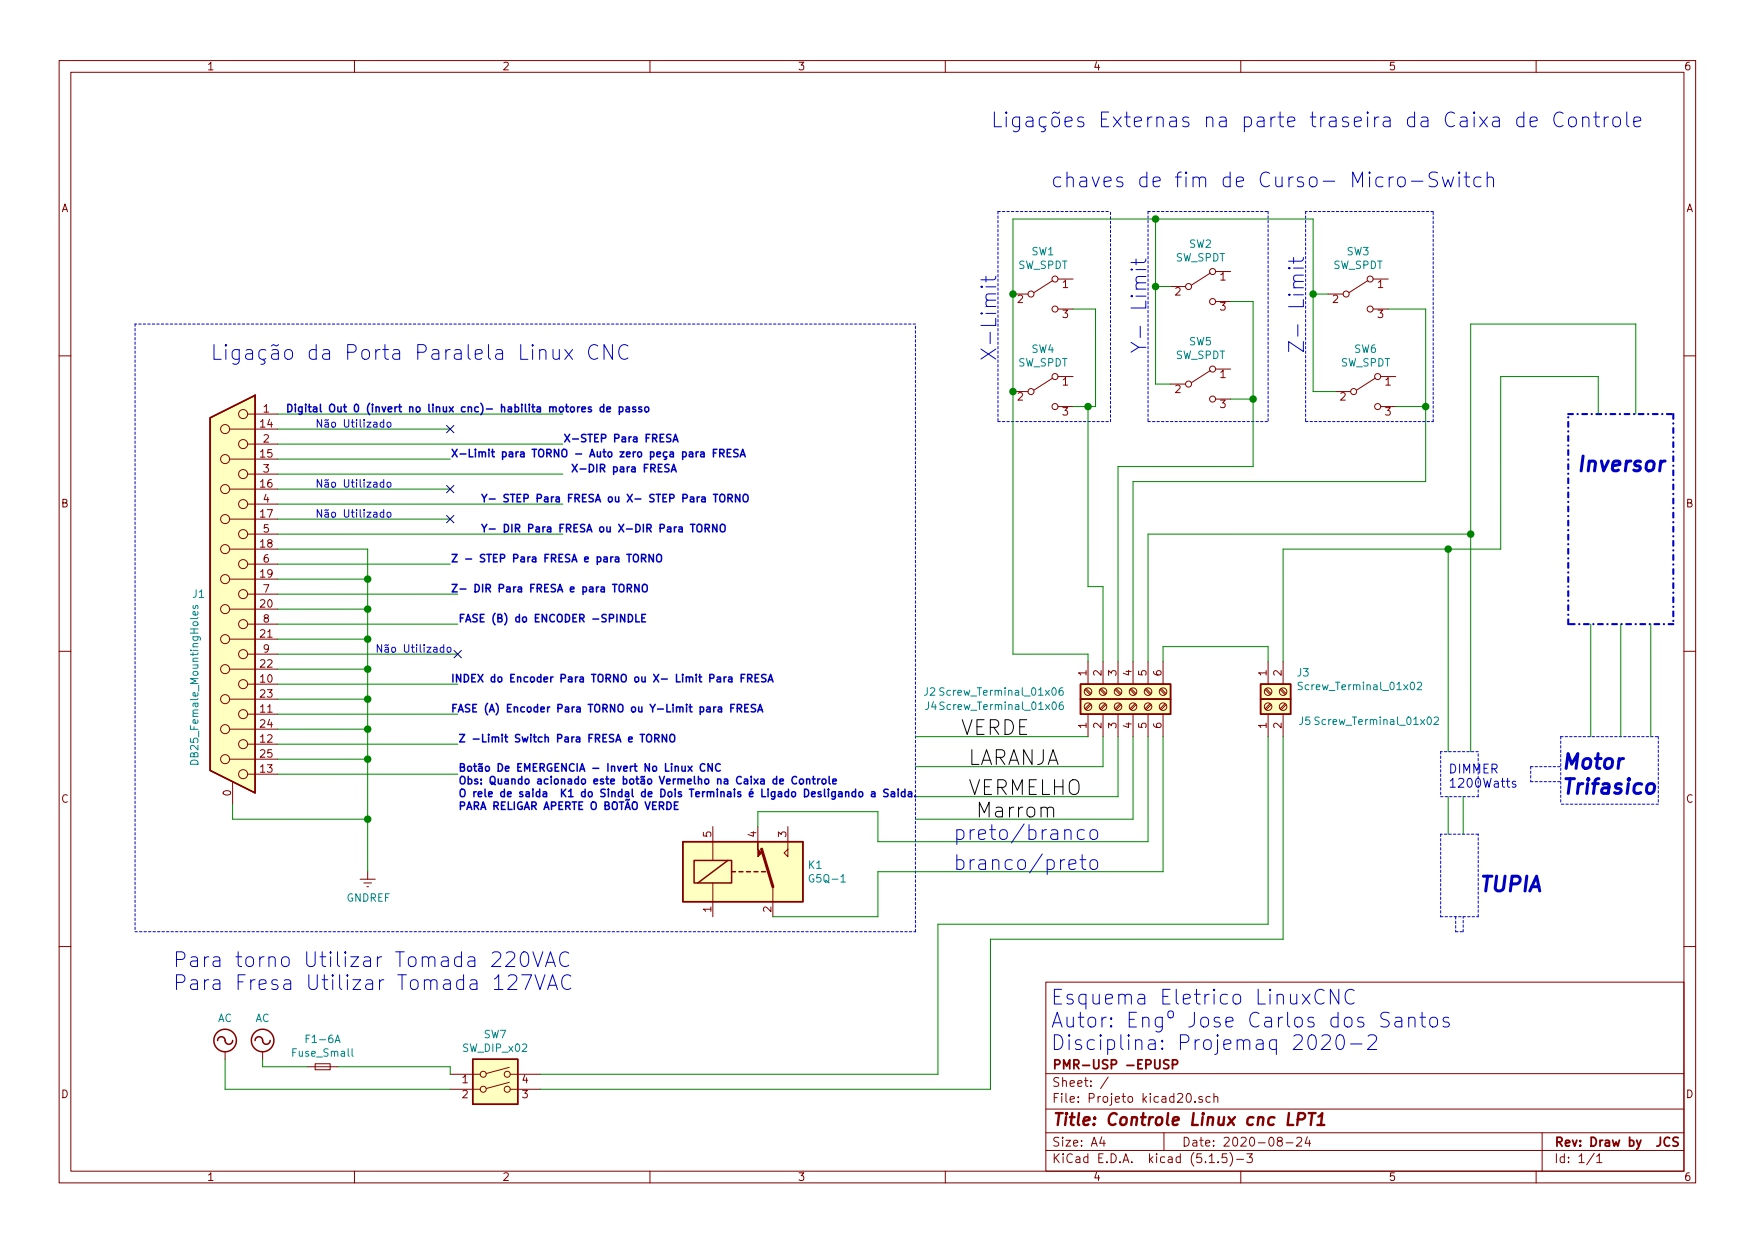
\includegraphics[width=\textwidth]{images/kicad-prof.jpg}
    \caption{Esquema elétrico fornecido pelo professor}
    \label{fig:prof_schematic}
\end{figure}

\begin{figure}[H]
    \centering
    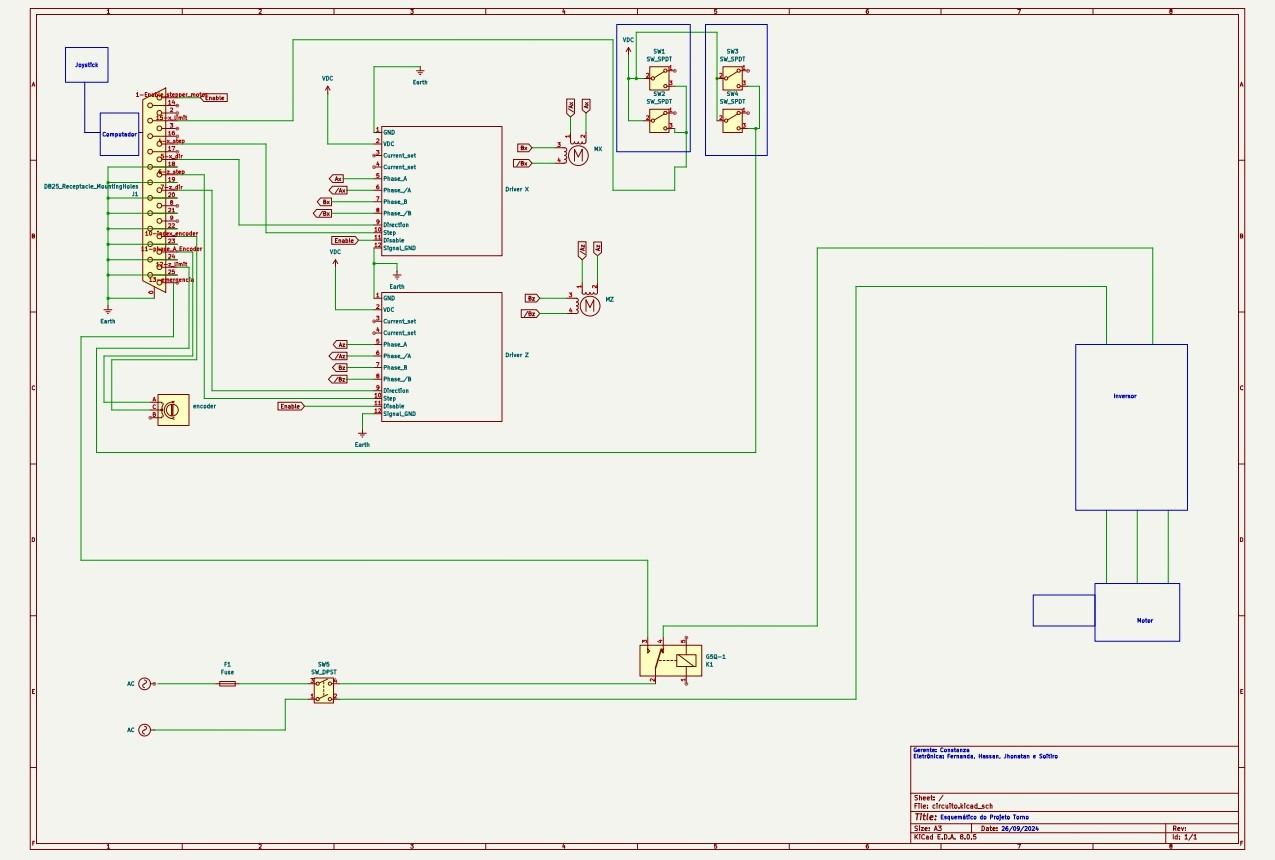
\includegraphics[width=\textwidth]{images/nosso-kicad.jpg}
    \caption{Esquema elétrico desenvolvido no KiCad}
    \label{fig:kicad_schematic}
\end{figure}

Algumas observações importantes incluem o fato de que o driver utilizado não estava disponível na biblioteca do KiCad, o que tornou necessário criá-lo seguindo as especificações técnicas de seu datasheet. No caso do encoder, foram consideradas apenas duas fases: a fase A e o index.

Para evitar "poluição visual", adotaram-se etiquetas para referenciar as conexões. Para o inversor e o motor, foi feito um esboço simplificado dos componentes, já que as suas características específicas não estavam presentes na biblioteca.


\section{Levantamento da curva do motor de passo}


\subsection{Montagem para realizar o teste}

Para coletar os dados necessários para levantar a curva do motor de passo (Torque x Velocidade Linear):

\begin{itemize}
    \item O motor foi fixado na mesa com um sargento (o nosso grupo usou o motor responsável pela movimentação no eixo Z);
    \item A carga de latão foi encaixada no eixo do motor, de forma que um dos furos onde o parafuso será colocado coincida com o lado chanfrado do eixo do motor;
    \item Primeiro, com o auxílio de uma chave de fenda, colocou-se o parafuso no furo que coincide com o lado chanfrado do eixo do motor;
    \item Depois, fixou-se o segundo parafuso.
\end{itemize}

A Fig. \ref{fig:montagem-teste} mostra a montagem realizada para o teste.

\begin{figure}[H]
    \centering
    \begin{subfigure}{0.35\textwidth}
        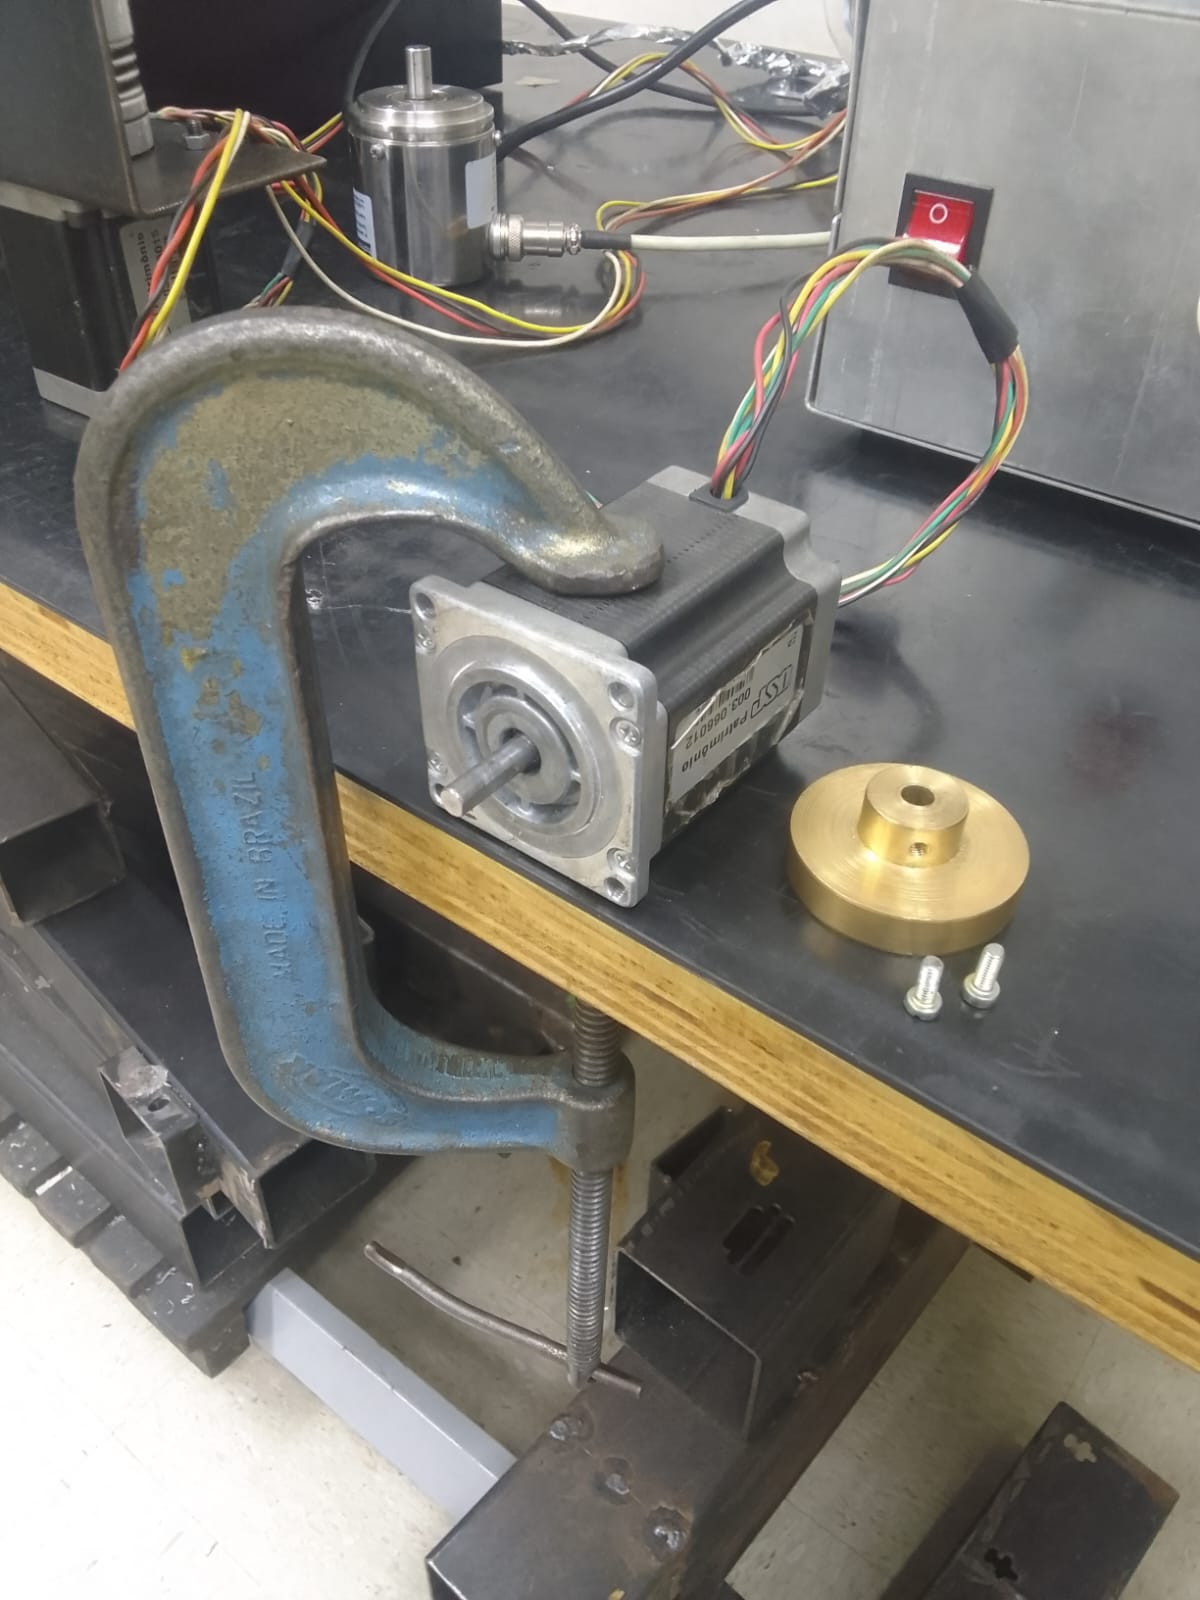
\includegraphics[width=\textwidth]{images/Eletrica/Figura1a.png}
    \end{subfigure}
    \begin{subfigure}{0.35\textwidth}
        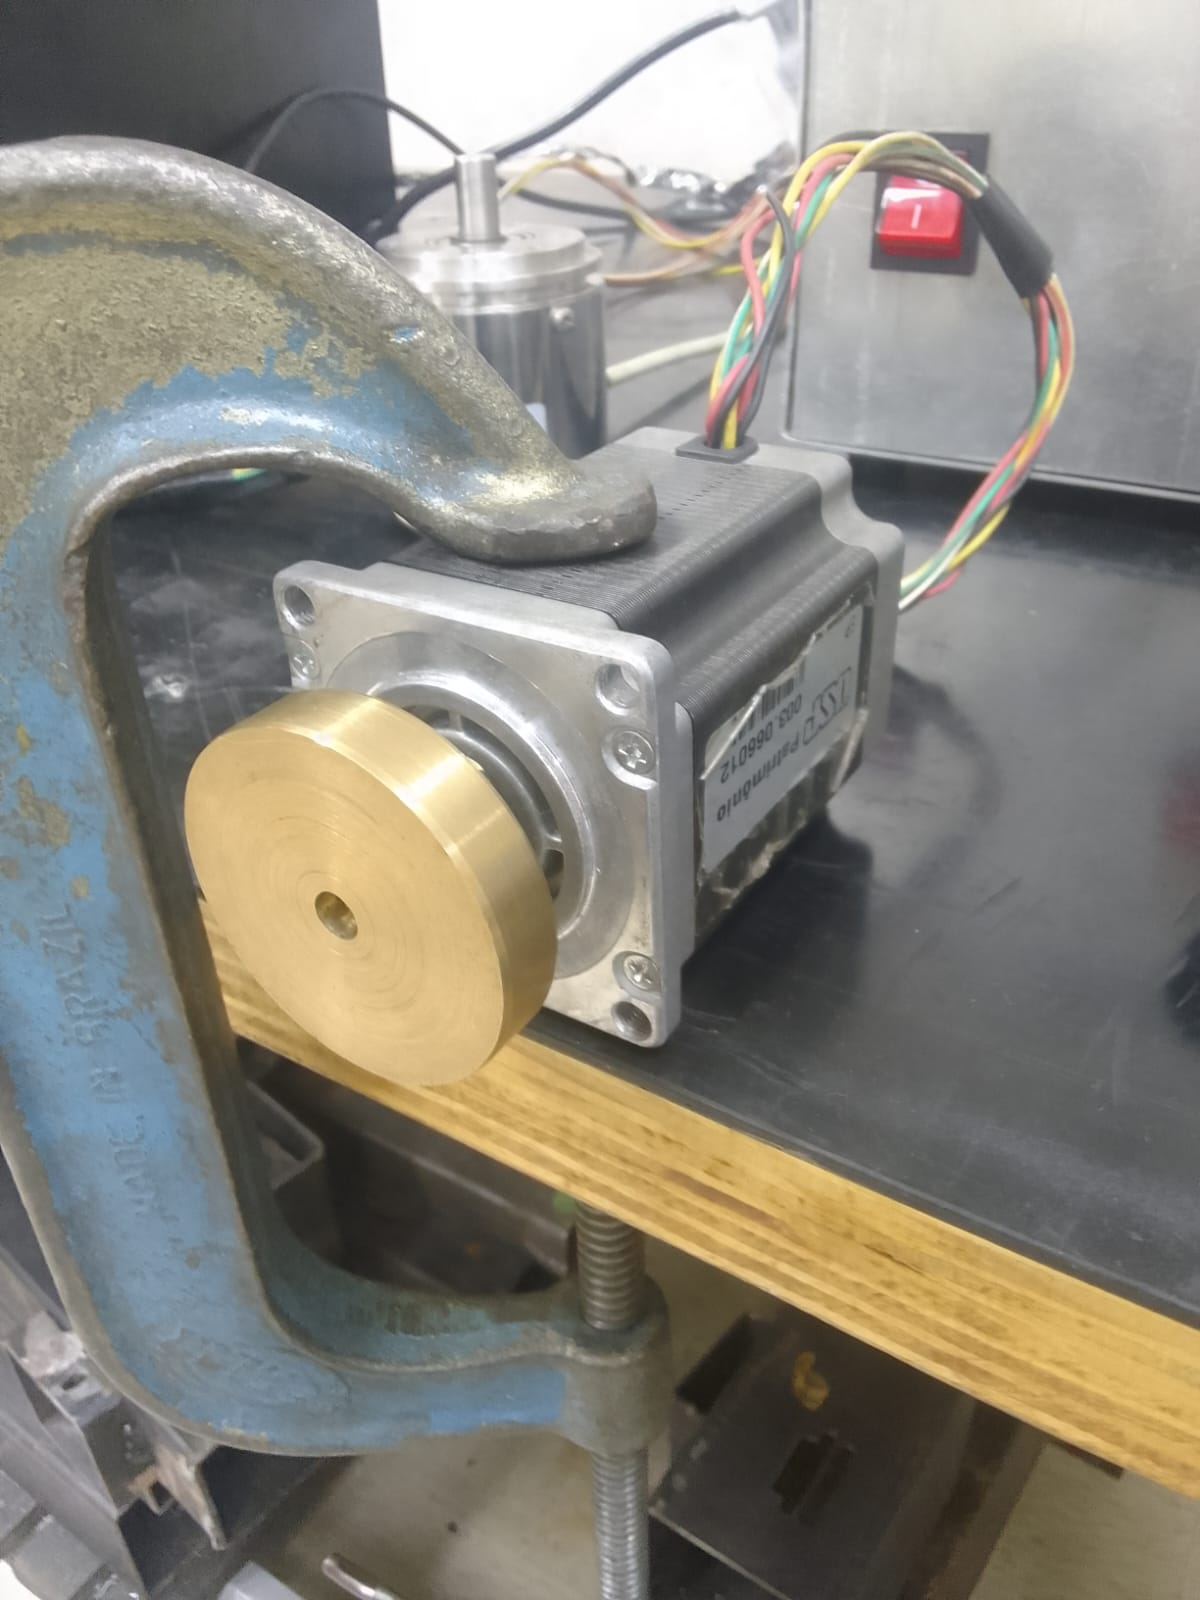
\includegraphics[width=\textwidth]{images/Eletrica/Figura1b.png}
    \end{subfigure}
    \caption{Motor de passo que controla o movimento no eixo Z antes e depois do acoplamento da carga de latão.}
    \label{fig:montagem-teste}
\end{figure}

\subsection{Passo a passo para abrir o Stepper Configuration Wizard e fazer os testes}

Concluída a montagem física para o levantamento da curva do motor, abriu-se o Stepconf -Stepper Configuration Wizard no LinuxCNC. A coleta de dados necessários para levantar os pontos da curva do motor é feita por esse aplicativo. As Figs \ref{fig:setup-curva-fig2}---\ref{fig:setup-curva-fig10} mostram a sequência de telas que aparecem até podermos realizar os testes.


Ao chegar na tela da Fig. \ref{fig:setup-curva-fig10}, temos um campo reservado para alterar a velocidade linear (mm/s) e outro para alterar a aceleração linear (mm/s2) da mesa deslizante.

Para cada velocidade escolhida, devemos anotar a máxima aceleração em que o motor ainda funciona sem perder o passo. A perda de passo é caracterizada pela parada da rotação, vibração e ruído do motor. 

Nosso grupo decidiu começar a coleta de dados na velocidade de 20 mm/s. Depois, foi-se acrescentando uma unidade ao valor da velocidade. A coleta terminou quando a velocidade atingiu 37.5 mm/s, o máximo valor suportado pelo LinuxCNC devido à limitação imposta pelas suas portas paralelas.


\subsection{Processamento para gerar a curva do motor}

Na mesa deslizante, o passo (5 mm) é a distância que a mesa percorre quando o fuso faz uma rotação completa. Assim, a divisão da aceleração linear ($mm/s^2$) pelo passo representa a percentagem de rotação do fuso em relação à sua rotação completa durante o intervalo de 1 $s^2$. Se multiplicarmos a razão por $2\pi$ rad, que é o valor de uma volta completa em radianos, encontramos a aceleração angular ($\text{rad}/s^2$):

\begin{equation}
    \alpha = 2\pi \frac{a_{\textbf{linear}}}{\textbf{passo}}
    \label{eq:alpha}
\end{equation}

O torque (Nm) é resultado da multiplicação do momento de inércia de massa (Kgm$^2$) da carga que foi acoplada no eixo do motor pela aceleração angular encontrada pela Eq. \ref{eq:alpha}:

\begin{equation}
    T = J\alpha
    \label{eq:torque}
\end{equation}

Para encontrar o momento de inércia de massa, vamos usar o modelo de cilindro oco (Fig. \ref{fig:cilindro-oco}), cuja expressão está na Eq. \ref{eq:modelo-cilindro}. 

\begin{figure}
    \centering
    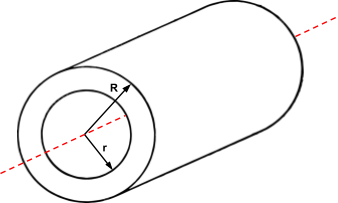
\includegraphics[width=0.6\linewidth]{images/Eletrica/Figura11.png}
    \caption{Modelo do cilindro oco, para cálculo do momento de inércia de massa.}
    \label{fig:cilindro-oco}
\end{figure}

\begin{equation}
    J = \frac{M}{2}(R^2 + r^2)
    \label{eq:modelo-cilindro}
\end{equation}

A carga de latão é modelada como dois cilindros ocos concêntricos, desprezando-se os dois furos para os parafusos e os próprios parafusos. O $r$ é o raio do furo central da carga e é igual para os dois cilindros ocos, diferentemente dos raios externos $R_1$ e $R_2$. As massas $M_1$ e $M_2$ de cada cilindro oco são calculadas conhecendo-se a densidade do latão e o volume calculado dos respectivos cilindros.

\noindent Dados do cilindro 1 (menor):

\begin{itemize}
    \item $r$ = 3.17 mm
    \item $R_1$ = 10.05 mm
    \item $h_1$ = 10.24 mm (altura do cilindro)
\end{itemize}

\noindent Dados do cilindro 2 (maior):

\begin{itemize}
    \item $r$ = 3.17 mm
    \item $R_2$ = 23.83 mm
    \item $h_2$ = 10 mm
\end{itemize}

\noindent A densidade do latão foi considerado como $\rho = 8500 \text{Kg/m}^3$.

Dessa forma, utilizando as expressões das Eqs. \ref{eq:massa}, \ref{eq:volume} e \ref{eq:modelo-cicindro}, foi possível obter os dados necessários, apresentados na Tab. \ref{tab:tab-dados-inercias}.

\begin{equation}
M = \rho V
    \label{eq:massa}
\end{equation}

\begin{equation}
V = \pi (R^1 - r^2)h
    \label{eq:volume}
\end{equation}

\begin{table}[H]
    \centering
    \caption{Dados necessários para cálculo do torque}
    \begin{tabular}{|c|c|c|}\hline
        Propriedade&Cilindo 1&Cilindo 2\\\hline
        Volume& $2.92597\dot10^{-6}$ m$^3$ &$1.75244\dot10^{-5}$ m$^3$\\\hline
        Massa&$2.4871\dot 10^{-2}$ kg&$1.4896\dot 10^{-2}$ kg\\\hline 
        Momento de Inércia&$1.381\dot10^{-6}$ kgm$^2$ &$ 4.304\dot10^{-5}$ kgm$^2$\\\hline
    \end{tabular}
    \label{tab:tab-dados-inercias}
\end{table}

A Tab. \ref{tab:valores-v-torques} mostra a velocidade linear e a máxima aceleração linear antes do motor perder o passo. Esses são dados anotados, enquanto $\alpha$ (aceleração angular) e torque são valores calculados.

\begin{table}[H]
    \centering
    \begin{tabular}{|c|c|c|c|}
    \hline
    \textbf{Velocidade (mm/s)}&\textbf{Aceleração (mm/s$^2$)}&\textbf{Alfa (rad/s$^2$)}&\textbf{Torque (Nm)}\\\hline
    20 & 6870 & 8633,10 & 0,383817 \\ \hline
    21 & 2390 & 3003,36 & 0,133526 \\ \hline
    22 & 2025 & 2544,69 & 0,113432 \\ \hline
    23 & 1735 & 2180,27 & 0,096932 \\ \hline
    24 & 1700 & 2136,28 & 0,094977 \\ \hline
    25 & 1655 & 2079,73 & 0,092462 \\ \hline
    26 & 1710 & 2148,85 & 0,095535 \\ \hline
    27 & 1715 & 2155,13 & 0,095871 \\ \hline
    28 & 1750 & 2199,11 & 0,097770 \\ \hline
    29 & 1715 & 2155,13 & 0,095815 \\ \hline
    30 & 1120 & 1407,43 & 0,062573 \\ \hline
    31 & 1800 & 2261,95 & 0,100065 \\ \hline
    32 & 1855 & 2331,06 & 0,103636 \\ \hline
    33 & 1875 & 2356,19 & 0,104754 \\ \hline
    34 & 40 & 50,27 & 0,002235 \\ \hline
    35 & 1070 & 1344,60 & 0,059779 \\ \hline
    36 & 1870 & 2349,91 & 0,104477 \\ \hline
    37 & 895 & 1124,69 & 0,050032 \\ \hline
    37,5 & 1245 & 1564,51 & 0,069556 \\ \hline
    \end{tabular}
    \caption{Valores encontrados de velocidade e aceleraçao lineares e valores calculados de aceleração angular e torque.}
    \label{tab:valores-v-torques}
\end{table}

Possuindo os dados de torque correspondentes a cada velocidade, foi possível plotar a “curva” do motor (Fig. \ref{fig:curva-motor}).

\begin{figure}[H]
    \centering
    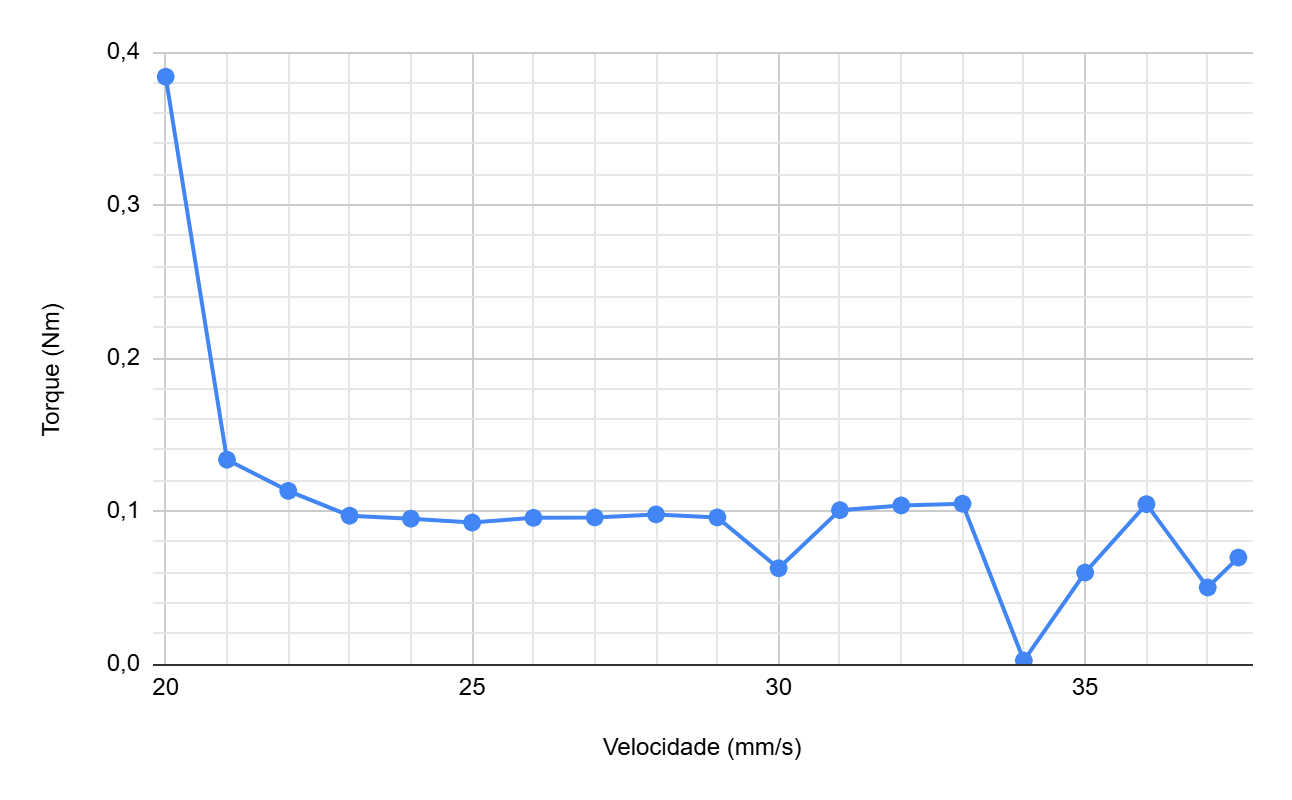
\includegraphics[width=0.85\linewidth]{images/Eletrica/Figura12.png}
    \caption{Gráfico do Torque (Nm) x Velocidade Linear (mm/s)}
    \label{fig:curva-motor}
\end{figure}

Adicionalmente, a planilha utilizada para registrar tais valores, assim como cálculos e plotagem do gráfico pode ser encontrada no link a seguir:  \url{https://docs.google.com/spreadsheets/d/1jPysggAJq_oss58Nr7ke5LIBtbU1b9r-ls-9ijTzHxM/edit?gid=0#gid=0}.


\section{Medição da Precisão e Acurácia}
\subsection{Metodologia} 
Primeiramente, é escolhida uma posição de origem para a mesa, na qual o relógio comparador é posicionado. A partir disso, a ela é deslocada a uma distância pré-determinada da origem e o comando de "home" é dado para que ela retorne a origem. Assim, o relógio mede a diferença entre a posição teórica (distância percorrida pela mesa) e sua posição real.

Esse procedimento foi realizado para duas posições teóricas, 100mm e 60mm para o eixo Z e 60mm e 30mm para o eixo X, com 5 medições para cada e velocidade de 200mm/s.

Uma vez que a acurácia é a proximidade entre o valor obtido experimentalmente e o valor verdadeiro na medição de uma grandeza física, ela foi calculada pela subtração da média das medições pelo valor real. Já a precisão, que significa grau de variação que surge a partir de diferentes medições, foi medida pelo desvio padrão entre as medições

\subsection{Resultados} 
Assim, após as medições, os resultados obtidos foram: 

% Tabela para o Eixo Z
\begin{table}[H]
\centering
\caption{Resultados das medidas no Eixo Z}
\begin{tabular}{|c|c|c|c|}
\hline
\multicolumn{2}{|c|}{Distância [mm] 100} & \multicolumn{2}{|c|}{Distância [mm] 60} \\ \hline
Número & Medidas [mm] & Número & Medidas [mm] \\ \hline
1 & 100.041 & 1 & 60.031 \\ \hline
2 & 100.042 & 2 & 60.030 \\ \hline
3 & 100.040 & 3 & 60.030 \\ \hline
4 & 100.040 & 4 & 60.031 \\ \hline
5 & 100.039 & 5 & 60.030 \\ \hline
Precisão & 0.001140175 & Precisão & 0.000547723 \\ \hline
Acurácia & 0.0404 & Acurácia & 0.0304 \\ \hline
\end{tabular}
\end{table}

% Tabela para o Eixo X
\begin{table}[H]
\centering
\caption{Resultados das medidas no Eixo X}
\begin{tabular}{|c|c|c|c|}
\hline
\multicolumn{2}{|c|}{Distância [mm] 60} & \multicolumn{2}{|c|}{Distância [mm] 30} \\ \hline
Número & Medidas [mm] & Número & Medidas [mm] \\ \hline
1 & 60.039 & 1 & 30.030 \\ \hline
2 & 60.038 & 2 & 30.031 \\ \hline
3 & 60.038 & 3 & 30.030 \\ \hline
4 & 60.038 & 4 & 30.030 \\ \hline
5 & 60.038 & 5 & 30.030 \\ \hline
Precisão & 0.000447214 & Precisão & 0.000447214 \\ \hline
Acurácia & 0.0382 & Acurácia & 0.0302 \\ \hline
\end{tabular}
\end{table}
